\documentclass[11pt,letterpaper]{article}
\usepackage[T1]{fontenc}
\usepackage[utf8]{inputenc}
\usepackage{lmodern,amsmath,amssymb,amsthm,mathtools}
\usepackage[margin=1in]{geometry}
\usepackage{microtype,booktabs,longtable,array,enumitem,xcolor,graphicx}
\usepackage{listings,fancyhdr}
\usepackage[colorlinks=true,linkcolor=blue!45!black,citecolor=blue!45!black,urlcolor=blue!55!black,breaklinks=true]{hyperref}
\setlength{\headheight}{14pt}
\pagestyle{fancy}\fancyhf{}
\fancyhead[L]{\small Finite geometry for adaptive contraction}
\fancyhead[R]{\small ProveIt research iteration}
\fancyfoot[C]{\thepage}
\setlength{\emergencystretch}{3em}
\setlength{\parskip}{3pt}
\setlist{itemsep=3pt,topsep=5pt}
\allowdisplaybreaks[2]
\newtheorem{theorem}{Theorem}[section]
\newtheorem{lemma}[theorem]{Lemma}
\newtheorem{proposition}[theorem]{Proposition}
\newtheorem{corollary}[theorem]{Corollary}
\theoremstyle{definition}\newtheorem{definition}[theorem]{Definition}
\theoremstyle{remark}\newtheorem{remark}[theorem]{Remark}
\newcommand{\poly}{\operatorname{poly}}
\newcommand{\K}{\mathcal K}
\newcommand{\pc}{\operatorname{popcount}}
\newcommand{\ceil}[1]{\left\lceil #1\right\rceil}
\newcommand{\floor}[1]{\left\lfloor #1\right\rfloor}
\newcommand{\F}{\mathbb F}
\newcommand{\pin}{\texttt{73dfb5e5ab6e91bd7375e5b97ef85d7e1cc8e81d}}
\newcommand{\anthpin}{\texttt{1a6eee293b9e00cb432eef6018a21f523623a9af}}
\lstset{basicstyle=\ttfamily\small,columns=fullflexible,breaklines=true,frame=single,framerule=.3pt}
\newcommand{\NewTimeBound}{30.692}
\newcommand{\NewSpaceBound}{29.467}
\newcommand{\NewTimeDisplay}{30.691338}
\newcommand{\NewSpaceDisplay}{29.466030}

\hypersetup{pdftitle={Finite Geometry for Adaptive Contraction: A Certified Improvement and the Remaining Order Barrier},pdfauthor={Research prepared for Vladimir Reshetnikov}}
\title{\textbf{Finite Geometry for Adaptive Contraction}\\[5pt]
\large A certified improvement beyond the twenty-nine reviewed SAT packets\\
and the remaining obstacle to a smaller exponent order}
\author{Research prepared for Vladimir Reshetnikov}
\date{October 26, 2026 (Pacific date)}
\begin{document}
\maketitle
\begin{abstract}
We review twenty filed refinement packets and all nine newer archives at
the pinned ProveIt snapshot, together with the public Anthropic proof supplied
during this investigation. The newest comparable generic cached bound is
$30.891018920366\ldots$ in the coefficient of $s/\sqrt{\log_2 s}$,
with space coefficient $30.753912832055\ldots$.
We give a new finite-geometric construction of adaptive contraction trees.
The four parallel classes of the affine plane $\F_3^2$ yield a sharp local
coefficient $1/\sqrt3$; a short Gram-matrix argument pays for every internal
table construction, not only the final multiplication. Together with a
second certified tree family and a fully paid recursion, the resulting
normalized time coefficient is at most \NewTimeBound, with space coefficient
at most \NewSpaceBound, for all sufficiently large inputs.
These are improvements of explicit asymptotic upper bounds. The algorithm
uses subexponential space and retains the existing reductions and exact
matrix-multiplication interface. It does not change the unrestricted SAT
order $n\log\log n/\sqrt{\log n}$, and does not claim the requested
logarithmic-order breakthrough. We also prove a scoped obstruction to a
direct odd-prime replacement and extend the known binary-separator witness
to unbalanced trees at the relevant arities. Exact checkers, a finite
contraction prototype, provenance records, and reproducible results accompany
the report. The new refinements are not Lean formalized.
\end{abstract}
\clearpage
\setcounter{tocdepth}{2}
\tableofcontents
\newpage
\section{Outcome, comparison, and scope}

There is a concrete new algorithmic ingredient in this iteration: select
contraction trees from parallel classes of a finite affine plane. This
gives a uniform bound over every exact mode-budget allocation, including
allocations concentrated on particular pairs. Its geometric overlap
properties control the maximum over all table-building operations.

The distinction between an improved exponential coefficient and a smaller
exponent order is essential. Our normalized guarantee has the form
\[
 T(s,\mathcal L)\le (s+\mathcal L)^{O(1)}
 2^{(C_T+o(1))s/\sqrt{\log_2s}},\qquad
 S(s,\mathcal L)\le (s+\mathcal L)^{O(1)}
 2^{(C_S+o(1))s/\sqrt{\log_2s}}.
\]
Here $s$ is a normalized Boolean-wire budget and $\mathcal L$ is the
description length. Neither coefficient is a coefficient per SAT variable.
The best polynomial-space branch remains available separately. This report
does not assert a new polynomial-space coefficient.

\begin{center}
\begin{tabular}{p{8.0cm}rr}
\toprule Generic normalized branch & Time coefficient & Space coefficient\\
\midrule
Best filed cached branch, before the nine arrivals &35.354588&34.274803\\
Best incoming cached branch &30.891019&30.753913\\
New certified cached branch &\NewTimeDisplay&\NewSpaceDisplay\\
Best incoming polynomial-space branch &46.184846&polynomial\\
\bottomrule
\end{tabular}
\end{center}
The first and second rows are the explicit certificates in
\cite{tree,portfolio}. The last row is \cite{flags}. All use the generic
maximum-degree promise $\ceil{s^{9/10}}$. Smaller numbers obtained under
stronger degree promises do not compete on this same input class.
An unspecified big-$O$ constant in another algorithm cannot be ranked against
these displayed coefficients. Nor are the conditional $n/\log n$ targets
proved algorithms that our result dominates.

For the two explicit asymptotic upper-bound expressions being compared,
reducing $C_T$ by a positive constant reduces their ratio by an exponential
factor on the $s/\sqrt{\log s}$ scale. It does not prove that an older
implementation actually requires its stated upper bound, and it is not a
measured SAT speedup.

\subsection{Frozen repository review}
The initial review pin is \pin. At that pin, the two requested directories
contained twenty filed packets and nine additional ZIPs. All nine ZIPs were retrieved at immutable
Git identities, checked against their Git blob hashes and ZIP integrity, and
extracted into separate directories. The report sources, status files, and
relevant algorithms were inspected; imported verification scripts were not
treated as proofs merely because their outputs were bundled.

\begin{center}\small
\begin{tabular}{p{3.1cm}p{10.8cm}}
\toprule Commit & Relevant change\\\midrule
\texttt{2b925d8800cd} & First seven refinement packets placed in the project.\\
\texttt{3e096089911f} & OpenAI preprint vendored from the pinned upstream source.\\
\texttt{45233238aebf} & First-round strongest-claims summary.\\
\texttt{6d3adc450615} & Eight second-round packets placed.\\
\texttt{450252e9d86c} & Five third-round packets placed; two omitted replay scripts restored.\\
\texttt{b9941a7396e4} & Nine newer SAT packets added to \path{docs/incoming}.\\
\texttt{73dfb5e5ab6e} & Reviewed repository head.\\
\bottomrule
\end{tabular}\end{center}
These dates are October 26 in Pacific time, although their UTC dates include
October 27. Immutable links and content hashes are supplied in the evidence
manifest. Repository placement is distinct from mathematical verification:
the ProveIt README explicitly treats the packets as externally supplied
research \cite{repo}.

\paragraph{Closing review of subsequent commits.}
Before delivery, commit \texttt{a7ae5ab55f96}
placed the same nine archives under \path{Research/}, and commit
\texttt{7de9d09fecd1} updated the Anthropic
formalization link. The latter is the closing repository head. All $443$
files actually placed in the nine new directories were compared with the
reviewed archive members by Git blob identity: none changed and no unexplained
new file appeared. The placement omitted $85$ of the $528$ archive members:
duplicate source/evidence copies and one checksum ledger. All $84$ omitted
duplicate copies were also matched to their recorded target Git blobs.
Of the $565$ pre-existing files, only the README and omission ledger changed;
no existing mathematical source was changed or deleted. At the closing
head all twenty-nine packets are filed, and \path{docs/incoming} contains
only its README. The mathematical comparison is unchanged; the archive
contains the complete old-to-current path map \cite{closing}.

\subsection{Twenty filed packets}
The following inventory identifies what must already be credited to the
reviewed corpus. ``PS'' means polynomial space; ``cached'' allows
subexponential space. Numerical entries are normalized-wire coefficients.

\small
\begin{longtable}{p{4.25cm}p{9.65cm}}
\toprule Packet & Contribution or limiting qualification\\\midrule\endfirsthead
\toprule Packet & Contribution or limiting qualification\\\midrule\endhead
\bottomrule\endfoot
\path{cauchy_mode_improvement} & Factorial Cauchy modes; weights $1+3q-2\pc(q)$; no order change.\\
\path{eth_contraction_improvements} & Sharper Hermite precision, streamed coefficient extraction; PS $648.44$.\\
\path{3sat_precision_refinement} & Leading precision $24MD/u\to6MD/u$; faster structured summation is conditional.\\
\path{sat_density_improvement} & Uniform density-aware SAT exponent; a genuine gain at some intermediate densities.\\
\path{eth_density_refinement} & Independent density refinement; local slope-four Smith valuations.\\
\path{3sat_refinement} & Scalar parity lift and smaller incidence-degree cap; second contraction lacks a closed representation.\\
\path{3sat_asymptotic_analysis} & Restricted barriers and explicit missing degree/compression interfaces.\\
\path{eth_asymmetric_packet_balancing} & Nearly lossless asymmetric packing and thin precision gaps; PS $76.909$.\\
\path{3sat_round2_refinement} & PS $84.066$; actual-domain gate and independent manuscript audits.\\
\path{eth_balanced_packing} & Deterministic balanced labels; PS $94.748$.\\
\path{eth_high_moment} & Independent $94.748$ certificate and low-degree variants.\\
\path{eth_matching_refinement} & Matching-potential packing; a third $94.748$ derivation.\\
\path{eth_packet_refinement} & Improved pair-load scale and padding; PS $95.664$.\\
\path{eth_recursive_refinement} & Residue-class mode refinement; PS $133.207$.\\
\path{eth_joint_cauchy} & Group-preserving full-block Cauchy modes; slope four; cached matrix option.\\
\path{sat_adaptive_contraction} & Streamed separators, PS $55.709$; adaptive cached $36.750$; exact kernels.\\
\path{sat_frontier_improvements} & Variable arity, PS $63.857$; cached $38.485$.\\
\path{subexponential_sat_frontier} & PS $63.852$; cached $37.930$; exact labeling and precision-peeling kernels.\\
\path{subexponential_sat_kernel_improvements} & Adaptive Smith, Gray, antipodal, and projective kernels; no smaller global order.\\
\path{subsat_contraction_tree} & Binary-built cached tables and exact ring bridge to a fast matrix backend; $35.355$.\\
\end{longtable}
\normalsize

\subsection{All nine incoming packets}
The newer arrivals materially change the benchmark. In particular it would
be incorrect to compare this iteration only against the filed $35.355$ or
$55.709$ figures.
\begin{center}\small
\begin{tabular}{p{7.1cm}rrr}
\toprule Archive stem & PS time & Cached time & Cached space\\\midrule
\path{3sat_round3_frontier_20261027} &63.75736&37.93011&33.62304\\
\path{ETH_Adaptive_Exact_Kernels_2026-10-27} &55.33162&35.07061&33.99950\\
\path{eth_adaptive_schedules_2026-10-26} &63.78117&37.59170&33.62304\\
\path{sat_adaptive_bounds_2026-10-26} &46.18485&34.32528&34.02418\\
\path{sat_adaptive_frontier_2026-10-26} &50.30469&31.25240&31.25240\\
\path{sat_adaptive_matrix_partition_2026-10-26} &50.21043&34.32528&34.02418\\
\path{sat_adaptive_tree_certificate_2026-10-26} &---&30.89102&30.75391\\
\path{subexponential_sat_adaptive_four_2026-10-26} &50.39373&32.91581&31.66171\\
\path{subsat_rectangular_2026-10-26} &53.97753&33.99389&33.99372\\
\bottomrule
\end{tabular}\end{center}
The adaptive-four packet also gives a slightly faster optional backend
variant; it remains above the best incoming generic cached bound. Low-degree
specializations are retained as separate branches. All nine incoming packets
retain the general SAT logarithmic order. Several already analyze precision
peeling, asymmetric Hermite multiplicities, conserved incidence degree, and
full-table barriers. Those observations are not claimed as new here.

\subsection{The SAT order that remains established}
With the imported reductions, the strongest proved order in the reviewed
corpus for fixed clause width is
\begin{equation}\label{eq:density-envelope}
 (n+m)^{O_k(1)}
 2^{O_k\!\left(\frac{n}{\sqrt{\log n}}
 \min\{\log(2+m/n),\log\log n\}\right)}.
\end{equation}
The direct clause-count branch can also be retained when it is smaller.
At fixed density this gives exponent $O_k(n/\sqrt{\log n})$;
at $m=\Theta(n\log\log n)$ it gives
$O_k(n\log\log\log n/\sqrt{\log n})$; in the unrestricted worst case
it gives $O_k(n\log\log n/\sqrt{\log n})$ \cite{density,upstream}.
The new contraction coefficient changes constants after applying these
reductions. It does not replace the square-root logarithm by a logarithm.

\section{Exact interface and paid contraction costs}
\label{sec:interface}

\subsection{Imported algebra and packing}
We use the same normalized problem as the current best generic packets.
The input is a bipartite Boolean tensor network with at most $s$ edges,
maximum degree at most $\ceil{s^{9/10}}$, and entries in
\[
 (\mathbb Z/2^{P_0}\mathbb Z)[V]/(V^\ell),\qquad 1\le P_0,\ell\le s.
\]
Entry evaluation has time $(s+\mathcal L)^{O(1)}2^{O(s^{9/10})}$ and
polynomial space, with fixed interface constants. The unchanged contraction
proof works in a polynomial-rank extension ring with an irreducible residue
polynomial of degree $O(\log s)$. Tensor descriptions retain their specified
creation precision and canonical entry representatives. Lifting those
representatives is not assumed to preserve ring operations.

The imported ingredients are exact Cauchy deformation and recovery,
asymmetric near-unit padding, full-orientation Cauchy modes, and recursively
evaluable group factors \cite{upstream,asymmetric,joint,portfolio}. This
report alters how the finite group-factor sum is evaluated. It is not an
independent proof of the entire upstream SAT algorithm.

At an active call use wire budget $M$, group count $r$, taper length $u$,
cumulative packet exponent $a$, a valuation $i<u$, and $D=2^{a-i}$.
The common interface supplies
\begin{align}
 p_t&\le(6+o(1))MD/u,\label{eq:working-precision}\\
 M_{\rm child}&\le(2/r+o(1))M.\label{eq:child-size}
\end{align}
For each directed pair of different groups, the multiplicity of each mode
index $q$ is at most $(2+o(1))M/(r^2D)$ and its certified weight is
$a+1-i+4q-2\pc(q)$. All error terms are uniform on the fixed set of
arities and the active levels of the final schedule.

If $Q=r^a$ and $R,C$ bound the two sides' degrees, sufficient padding gates
are
\begin{equation}\label{eq:packing}
 QR/M=o(1),\quad Q^2C(\log s)^2/M=o(1),\quad 2^aQ^2/M=o(1).
\end{equation}
At the root both sides have degree at most $s^{9/10+o(1)}$. Subsequently
the old side retains that bound and the fresh side has degree at most
$2^{a_{d-1}+1}$. Section~\ref{sec:schedule} checks these gates before
using the child-size conclusion.

\subsection{Exact mode lists and the entropy envelope}
Enumerate exact nonnegative pair budgets $b_{gh}$ with sum less than $p_t$.
There are polynomially many such arrays because $r$ is fixed and $p_t$ is
polynomial in $s$. Let $\mathcal I_{gh}$ be the finite list of mode
exponent tuples of exact weight $b_{gh}$. Empty lists contribute zero.
Put $h_{gh}=\log_2|\mathcal I_{gh}|$ and
\[
 \kappa=\frac{\pi\sqrt2}{\ln2},\qquad
 \K(M,u)=\kappa M/\sqrt u.
\]
The contribution of the budget array is exactly
\begin{equation}\label{eq:finite-sum}
 \sum_{\xi_{gh}\in\mathcal I_{gh}}
 \prod_{g=1}^r Z_g\bigl((\xi_e)_{e\ni g}\bigr).
\end{equation}
Each $Z_g$ entry requires a real recursive contraction; it is not a
unit-cost oracle.

For a fixed nonnegative directed weight vector $z$, the inherited bound is
\begin{equation}\label{eq:entropy}
 \sum_e z_eh_e\le
 \left(\frac{\|z\|_2}{r}+o(1)\right)\K(M,u).
\end{equation}
For clarity, its leading constant follows by lowering mode weights to
$1+4q-2\pc(q)$ and applying the generating-function estimate
\[
 \sum_{q\ge0}-\ln(1-e^{-\theta(1+4q-2\pc(q))})
 =\frac{\pi^2}{24\theta}+O(\log^2(2/\theta)).
\]
Using a common tilt $\theta/z_e$ gives leading natural-log bound
\[
 \theta p_t+\frac{\pi^2}{24\theta}
 \frac{(2+o(1))M}{r^2D}\sum_ez_e^2.
\]
Optimize in $\theta$, apply \eqref{eq:working-precision}, and divide by
$\ln2$. The logarithmic guard ensures that the residual term is lower order.
For a fixed finite family of vectors, the error is uniform. All adaptive
arguments below use such a finite family; no pointwise bound is silently
applied to an uncontrolled growing collection.

List sizes and indexing are explicit. The unbounded-knapsack recurrence
\[
 N(j,b)=N(j-1,b)+N(j,b-w_j),\quad N(0,0)=1
\]
with zero values for impossible budgets counts exact tuples. It also gives
rank/unrank and polynomial-delay enumeration. Budgets, list-count bit lengths,
and the number of mode types are polynomial in the original size parameter.

\subsection{Matrix operations and support vectors}
For disjoint group sets $A,B$ and $O=[r]\setminus(A\cup B)$, merging two
boundary tables has three independent index classes: pairs joining $A$ to
$O$, $A$ to $B$, and $B$ to $O$. Write their logarithmic dimensions as
$H_1,H_2,H_3$. Using the established strict rational matrix exponent
$\omega<12/5$ gives the upper exponent
\begin{equation}\label{eq:matrix-cost}
 H_1+H_2+H_3-\frac35\min(H_1,H_2,H_3)
 =\max_j\left(\frac25 H_j+\sum_{k\ne j}H_k\right).
\end{equation}
Square blocking proves this rectangular estimate. The cited matrix result
is stronger than needed; no newest-record assertion is necessary
\cite{matrix}.

The ring bridge is the one already established in \cite{tree,portfolio}.
Expand each ring entry into its polynomially many integer coordinates,
perform coordinate matrix products modulo sufficiently many ordinary primes
away from the fixed denominator exceptions of a rational bilinear algorithm,
reconstruct by CRT, apply the ring structure constants, and reduce modulo
$2^{p_t}$. All reconstruction bounds have polynomial bit length. This uses
neither division by a nonunit in the original ring nor a false field model
for that ring. The fast backend is a theoretical dependency; the small
prototype in this archive uses ordinary exact multiplication.

For an undirected pair $e=\{g,h\}$ put $g_e=h_{gh}+h_{hg}$. Multiply
\eqref{eq:matrix-cost} by five. Each operation supplies three vectors
$v\in\{0,2,5\}^{\binom r2}$, zero on edges internal to its three
parts, two on a discounted cross class, and five on the other classes.
A plan first divides the groups into three blocks, builds each block table
by binary merges, then contracts the final triangle. If $\mathcal V_j$ is
the complete support set for plan $j$, put
\[
 F_j(g)=\frac15\max_{v\in\mathcal V_j}v\cdot g.
\]
Every boundary table is the input or output of an operation. Its exponent
is a sum of two of the $H_i$, hence at most \eqref{eq:matrix-cost}.
Thus $F_j$ pays for all local time and storage after singleton caching.

\begin{lemma}[Paid adaptive support certificate]\label{lem:certificate}
For $q$ fixed plans on $r$ groups let
\[
 Q_* =\max_{v_j\in\mathcal V_j}\left\|\sum_{j=1}^qv_j\right\|_2^2,
 \qquad \beta_r=\frac{\sqrt{2Q_*}}{5qr},\qquad
 \alpha_r=\frac{\sqrt{2(r-1)}}r.
\]
Choosing a plan with smallest $F_j$ gives the recurrence
\begin{equation}\label{eq:paid-recurrence}
 T_d\le\poly(s)\left[
 2^{(\alpha_{r_d}+o(1))\K_d}T_{d+1}
 +2^{(\beta_{r_d}+o(1))\K_d}\right],
\end{equation}
and local storage at most $\poly(s)2^{(\beta_{r_d}+o(1))\K_d}$.
\end{lemma}
\begin{proof}
The minimum of the $F_j$ is at most their average, which equals
\[
 \frac1{5q}\max_{v_j\in\mathcal V_j}
 \left(\sum_jv_j\right)\cdot g.
\]
Give both directed orientations of an edge the weight
$(\sum_jv_j)_e/(5q)$ and apply \eqref{eq:entropy}. Its squared directed
norm is $2\|\sum_jv_j\|_2^2/(25q^2)$, giving $\beta_r$.
There are finitely many support tuples. The storage assertion follows
from the preceding input/output observation. Caching one group's entries
involves $2(r-1)$ incident directed pairs, giving $\alpha_r$; each entry
is charged its child contraction. The fixed number of groups is absorbed
by the polynomial factor.

Selection needs no real-number oracle. Compute
$\max_{v\in\mathcal V_j}\prod_e
(|\mathcal I_{gh}|\,|\mathcal I_{hg}|)^{v_e}$ and compare those
positive integers. Their bit lengths are polynomial. Sorted sequential
table scans and reshaping add only polynomial factors in index and record
length, so the analysis does not rely on free exponential random access.
\end{proof}

\section{The affine-plane contraction certificate}
\label{sec:affine}

\subsection{Four geometric plans}
Identify nine group labels with $(x,y)\in\F_3^2$, using integer label
$3x+y$. For each of the four linear forms
\[
 x,\qquad y,\qquad x+y,\qquad x+2y
\]
partition the points into the three level sets. Each set is a line of
three points. Within an ordered line $(a,b,c)$ first merge $b,c$, then
merge the result with $a$. Finally contract the three line tables.
There are six internal merges and one final triangle, hence $21$ support
vectors per plan.

\begin{center}\small
\begin{tabular}{cl}
\toprule Direction & Ordered line blocks\\\midrule
$x$ & $(0,1,2)\mid(3,4,5)\mid(6,7,8)$\\
$y$ & $(0,3,6)\mid(1,4,7)\mid(2,5,8)$\\
$x+y$ & $(0,5,7)\mid(1,3,8)\mid(2,4,6)$\\
$x+2y$ & $(0,4,8)\mid(2,3,7)\mid(1,5,6)$\\
\bottomrule
\end{tabular}\end{center}

\begin{figure}[ht]
\centering
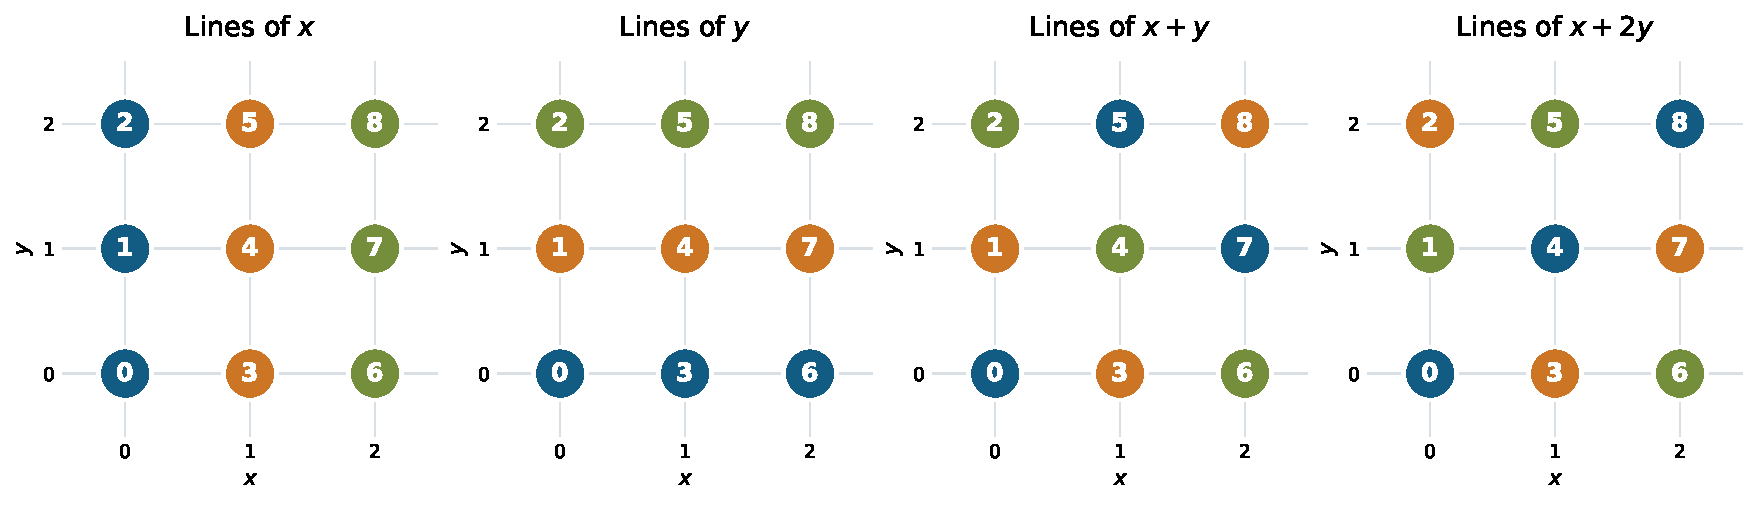
\includegraphics[width=.94\textwidth]{figures/affine_partitions.pdf}
\caption{The same nine groups in four partitions. Equal colors form a
line block. Every pair of distinct points lies together in exactly one
partition, and lines from different partitions meet in one point.}
\end{figure}

These balanced intersection properties are what an arbitrary handful of
permuted trees lacks. They control the overlap between \emph{all} operation
supports, including the operations used to build the tables.

\subsection{A short Gram certificate}
Classify an operation as $P$ (merge two points), $L$ (complete a line), or
$R$ (the root triangle). The following are exact maxima for these four
plans. A transverse pair means supports from different parallel classes.
\begin{center}
\begin{tabular}{crrr}
\toprule Type & $P$ & $L$ & $R$\\\midrule
Maximum single-support squared norm &354&458&486\\
\bottomrule
\end{tabular}\qquad
\begin{tabular}{c|rrr}
Maximum transverse inner product &$P$&$L$&$R$\\\hline
$P$&204&208&215\\
$L$&208&240&260\\
$R$&215&260&288
\end{tabular}
\end{center}
The single-support entries follow directly from the cross-class sizes.
For example, a line-completion operation has undirected class sizes
$2,6,12$, so its largest norm is $4\cdot2+25(6+12)=458$.
A root has three classes of nine edges, giving $9(4+25+25)=486$.
The transverse entries are exact nine-point incidence counts. The
independent checker reconstructs them from Cartesian edge classes.
For the theorem, a short geometric argument supplies slightly weaker
mixed bounds, all still strictly below $288$; no exhaustive computation
is needed for its principal inequality.

A $P$ profile is supported on edges incident to its chosen pair. An $L$
profile is supported on edges incident to its line, except for the edge
between the two points merged first. Transverse lines meet in one point.
Two $P$ supports therefore share at most nine edges, and a $P$ and an
$L$ share at most ten. Since coefficients are at most five, their inner
products are at most $225$ and $250$. In a $P$--$R$ comparison, the
selected points lie in distinct root blocks; eleven root-crossing edges
meet the pair, giving at most $275$.

Two full line-incidence sets share twelve edges: eight incident with their
intersection and four joining their remaining pairs. If the intersection
is not the singleton in at least one of the two line merges, an omitted internal edge is
shared, leaving at most eleven edges and bound $275$. Otherwise the
intersection is the singleton of both merges. Every possible discounted
class contains at least two shared edges; each has product at most ten
instead of twenty-five, so the bound is $300-30=270$.

For $L$--$R$, the transverse line meets each root block once. Root weights
sum to $48$ on its external incident edges and $12$ on its internal
triangle. The line profile omits an internal edge of root weight at least
two, so its undiscounted dot product is at most $5(60-2)=290$.
Its discounted class has root-weight sum at least four, reducing this
by at least $3\cdot4$ to $278$. Thus every mixed transverse inner
product is strictly less than $288$. The root-root case has the exact
geometric proof below. These arguments work for any ordering within a line.

\begin{theorem}[Sharp four-plan certificate]\label{thm:affine}
For the four affine-plane plans,
\[
 \max_{v_j\in\mathcal V_j}\left\|v_1+v_2+v_3+v_4\right\|_2^2=5400.
\]
Consequently their local coefficient in Lemma~\ref{lem:certificate} is
$\beta_9=1/\sqrt3$.
\end{theorem}
\begin{proof}
The Gram bounds give
\[
 \left\|\sum_jv_j\right\|_2^2
 =\sum_j\|v_j\|_2^2+2\sum_{j<k}\langle v_j,v_k\rangle
 \le4\cdot486+2\binom42\,288=5400.
\]
Every choice of four root supports attains equality. Here is a geometric
verification, also explaining why the constant is simple.
Let $C_j$ be the cross-edge set of direction $j$ and let $D_j$ join the
two parallel lines chosen for its discounted class. A root support is
$5\mathbf1_{C_j}-3\mathbf1_{D_j}$. For distinct directions,
\[
 |C_j\cap C_k|=18,\quad |D_j\cap C_k|=|C_j\cap D_k|=6,
 \quad |D_j\cap D_k|=2.
\]
The last identity counts the two diagonals of the affine $2$ by $2$
rectangle obtained by retaining two levels of each independent linear
form. Therefore every transverse root inner product is
$25\cdot18-15(6+6)+9\cdot2=288$. Each root norm is $486$.
Finally
\[
 \beta_9^2=\frac{2\cdot5400}{25\cdot4^2\cdot9^2}=\frac13.
\]
\end{proof}

As an additional independent check, all $21^4=194{,}481$ tuples were
enumerated with integer arithmetic. The sum of their squared norms is
$622{,}974{,}240$. Exactly $81=3^4$ tuples attain $5400$; every one
uses four root supports. The largest value involving an internal operation
is $5204$. These checks support the finite incidence table; they are not
samples of entropy vectors.

\subsection{Sharpness within this particular menu}
The coefficient is the exact minimax value for this four-plan support
model, not merely a convenient sufficient bound. Choose any root support
$v_j$ from each direction and set $g=\sum_jv_j$. Then
$\|g\|_2^2=5400$ and
\[
 v_j\cdot g=486+3\cdot288=1350\qquad(1\le j\le4).
\]
Thus every plan has $F_j(g)\ge270$. The averaging bound gives equality.
Assigning each directed orientation half the corresponding $g_e$ and
normalizing to the Euclidean entropy ball witnesses the coefficient
$1/\sqrt3$. This is not an optimality claim over all possible tree menus,
over actual realizable mode lists, or over SAT algorithms.

\subsection{A second finite certificate for the recursive bottleneck}
For thirteen groups use the following four plans. In each block, recursively
split the ordered list at its floor midpoint, build the two subblocks, and
merge. Finish with the three-block triangle.
\begin{center}\small
\begin{tabular}{cl}
\toprule Plan & Ordered blocks\\\midrule
1 & $(0,1,2,3,4)\mid(5,6,7,8)\mid(9,10,11,12)$\\
2 & $(12,10,1,6,4)\mid(9,0,3,8)\mid(5,2,7,11)$\\
3 & $(0,8,11,12,1)\mid(7,10,4,3)\mid(5,2,6,9)$\\
4 & $(1,7,0,6,9)\mid(5,10,11,3)\mid(12,8,4,2)$\\
\bottomrule
\end{tabular}\end{center}
The first three plans occur in the incoming certificate; adding the fourth
and certifying the complete new menu is the additional finite refinement.
There are eleven operations and $33$ profiles per plan. Direct exact
evaluation gives squared norm at most $1064$ for every single profile
and inner product at most $647$ for every pair from different plans.
Consequently
\[
 Q_{13}\le4\cdot1064+12\cdot647=12020,
 \qquad \beta_{13}^2=\frac{2\cdot12020}{25\cdot16\cdot169}
 =\frac{601}{1690}.
\]
Equality occurs when each final triangle discounts the class between its
two four-point blocks. The $6534=6\cdot33^2$ pairwise integer checks
and the matching witness suffice to certify this bound. Two independently
written programs also enumerate all $33^4=1{,}185{,}921$ tuples;
their squared-norm sum is $5{,}700{,}575{,}232$, with a unique maximizer.
No floating search result is used as a mathematical acceptance condition.

For completeness, the finite Gram calculation is exactly the following:
\begin{lstlisting}
for plan in plans:
    operations = binary_merges_inside_blocks(plan) + [final_triangle(plan)]
    profiles = [cross_class_weights(op, discount, high=5, low=2)
                for op in operations for discount in range(3)]
check(all(dot(v,v) <= 1064 for v in every_profile))
check(all(dot(v,w) <= 647 for v,w in different_plan_pairs))
check(dot(sum_of_four_displayed_root_profiles,
          sum_of_four_displayed_root_profiles) == 12020)
\end{lstlisting}
The supplied plans, midpoint rule, pair coordinates, and profile definition
fully specify this finite certificate.

\subsection{Why a better local bound is not enough}
The incoming best cached schedule has its maximum at the second recursion
stage, not at the root. Replacing its nine-group coefficient alone would
improve memory but leave the time coefficient $30.8910189\ldots$ unchanged.
The global construction must also improve that later bottleneck. The next
section includes the needed second certificate, its actual child-entry
costs, and an explicit feasible schedule. This prevents a local-only gain
from being reported as a global speedup.

\section{A fully paid recursion with the new certificates}
\label{sec:schedule}

The local affine-plane certificate becomes a global improvement only after
the expensive evaluation of the cached group functions is included. We use the explicit $9\to13\to7$ schedule below to improve the
second-stage bottleneck as well as the root. This section states all additional
resource assumptions and checks the complete recurrence.

\subsection{Normalized inherited interface}

Let $s\ge2$, $\lambda=\lceil\log_2s\rceil$, and let the initial
bipartite Boolean tensor network have at most $s$ wires and maximum degree
at most $\lceil s^{9/10}\rceil$. Its entries lie in
$(\mathbb Z/2^{P_0}\mathbb Z)[V]/(V^\ell)$ with $P_0,\ell\le s$.
Let $\mathcal L$ be its description length. The permitted original entry
procedures take $(s+\mathcal L)^{O(1)}2^{O(s^{9/10})}$ time and polynomial
space, with fixed exponents and constants. The ring extension, canonical
creation-time lifts, exact deformation, and Hermite recovery are the
inherited normalized interface of the reviewed packets. Thus the result
below is a proved refinement of that interface; it does not independently
verify the upstream exact-counting algorithm.

At an active call with $M$ wires, group count $r$, and taper length $u$,
write
\[
 \mathcal K(M,u)=\kappa\frac{M}{\sqrt u},\qquad
 \kappa=\frac{\pi\sqrt2}{\ln2}.
\]
The inherited full-Cauchy entropy estimate says that if $h_{gh}$ is the
base-two logarithm of the exact list cardinality on directed group pair
$(g,h)$, then for every fixed nonnegative weight vector $z$,
\[
 \sum_{g\ne h}z_{gh}h_{gh}
 \le\left(\frac{\sqrt{\sum_{g\ne h}z_{gh}^2}}r+o(1)\right)
       \mathcal K(M,u).
\]
Exact weight allocations have total below the polynomially bounded working
precision. Because only the three fixed group counts $9,13,7$ occur, there
are polynomially many such allocations. The local certificates from the
preceding section apply uniformly to each allocation.

There are $2(r-1)$ directed pairs incident to one group. Consequently the
total number of singleton-table entries, including the sum over all groups,
is at most
\[
 \operatorname{poly}(s)\,
 2^{(\alpha_r+o(1))\mathcal K(M,u)},\qquad
 \alpha_r=\frac{\sqrt{2(r-1)}}r.
\]
Every entry is computed by a recursive child contraction with at most
$(2/r+o(1))M$ wires. Charging these calls separately from the local tree
operations gives
\begin{equation}
 T_d\le \operatorname{poly}(s)
 \left[2^{(\alpha_{r_d}+o(1))\mathcal K_d}T_{d+1}
       +2^{(b_{r_d}+o(1))\mathcal K_d}\right],
 \qquad \mathcal K_d=\mathcal K(M_d,u_d).
 \label{eq:affine-paid-recurrence}
\end{equation}
The local coefficients used here are
\[
 b_9^2=\frac13,\qquad b_{13}^2=\frac{601}{1690},\qquad
 b_7^2=\frac{632}{1225}.
\]
The first two come from the new four-plan certificates. The last is the
fixed seven-group plan $(0,1,2)\mid(3,4)\mid(5,6)$: its integer operation
supports have maximum squared norm $316$, so its directed normalized
coefficient is $2\cdot316/(25\cdot7^2)$. The supplied checker verifies this
bound directly.

The matrix operations use the inherited exact integer-coordinate and CRT
bridge for a fixed rational matrix multiplication algorithm with exponent
strictly below $12/5$. Thus the proof pays for the arithmetic over the
source ring rather than assuming that the ring is a field. No fast matrix
multiplication backend or end-to-end contraction solver is implemented by
the certificate programs.

\subsection{An explicit strict rational schedule}

Choose
\begin{align*}
 r_0&=9,& \eta_0&=\frac{15773}{1000000},\\
 r_1&=13,&\eta_1&=\frac9{800},\\
 r_d&=7\quad(d\ge2),&
 \eta_d&=\frac{8597}{1800000}
                   \left(\frac49\right)^{d-2}\quad(d\ge2).
\end{align*}
Put
\[
 u_d=\lfloor\eta_d\lambda\rfloor,\qquad
 B=\lceil6\log_2\lambda\rceil,\qquad
 a_d=\sum_{j=0}^d(u_j+B),\qquad
 H=\left\lceil\frac{s}{\lambda^{3/4}}\right\rceil.
\]
Use the inherited near-unit padding with relative slack $\lambda^{-3}$.
Calls with $M\le H$ are evaluated directly. For sufficiently large $s$
every active $u_d$ is positive; a fixed exceptional initial range is handled
by exhaustive contraction. The exact capacity sums are
\[
 \eta_0+\eta_1=\frac{27023}{1000000},\qquad
 \sum_{d\ge0}\eta_d=\frac{1781}{50000}.
\]

The following integer inequalities give rational upper bounds for every
logarithm needed in the packing proof:
\[
 9^{100000}<2^{316993},\qquad
 13^{100000}<2^{370044},\qquad
 7^{100000}<2^{280736}.
\]
They are checked using exact arbitrary-precision integers. Their respective
upper bounds for $\log_2 9$, $\log_2 13$, and $\log_2 7$ are
$316993/100000$, $370044/100000$, and $280736/100000$.

At the root both old sides have degree exponent $9/10$. At a later depth,
one side has that same old-degree bound, whereas the fresh side has degree
at most $2^{a_{d-1}+1}$. The asymmetric packing requirements are, up to
polylogarithmic factors, $Q^2\Delta$ at the root and $QR$, $Q^2C$,
$2^aQ^2$ later, with $Q=r^a$, retained degree $R\le s^{9/10+o(1)}$,
and fresh degree $C\le2^{a_{d-1}+1}$. The dominant margins are
\begin{center}
\begin{tabular}{lll}
\hline
Stage & Upper bound on the leading exponent & Margin below one\\
\hline
Root & $\displaystyle \frac9{10}
       +2\frac{15773}{1000000}\frac{316993}{100000}$
     & $\displaystyle\frac{69411}{50000000000}$\\[5pt]
Depth one & $\displaystyle \frac9{10}
       +\frac{27023}{1000000}\frac{370044}{100000}$
     & $\displaystyle\frac{75247}{25000000000}$\\[5pt]
Tail & $\displaystyle \frac9{10}
       +\frac{1781}{50000}\frac{280736}{100000}$
     & $\displaystyle\frac{287}{156250000}$\\
\hline
\end{tabular}
\end{center}
Every margin is strictly positive. The secondary fresh-side and packet
terms are controlled by
\[
 \frac{1781}{50000}
       \left(2\frac{370044}{100000}+1\right)<1.
\]
The fresh packet degree exponent is at most $1781/50000+o(1)<9/10$.
The smallest displayed power gaps are of order $10^{-6}$. They certify
eventual asymptotic feasibility, with no useful practical-size threshold
claimed here. This is one reason the coefficient comparison should not
be interpreted as a benchmark prediction.

\subsection{Uniformity, depth, and precision}

We give a bootstrap rather than using a depth bound as an unproved premise
of packing. Consider hypothetical active tail depths up to
$3\log_3\lambda/4+O(1)$. On this range,
\[
 u_d\ge\lambda^{\epsilon+o(1)},\qquad
 \epsilon=1-\frac{3\ln(9/4)}{4\ln3}>0.
\]
For example, positivity follows from $(9/4)^3<3^4$.
The cumulative guard adds only $O((\log\lambda)^2)$ to $a_d$.
The positive fixed margins above absorb this guard, all packing
polylogarithms, and $s/M<\lambda^{3/4}$. Padding is therefore valid
throughout the hypothetical range, with relative error
$O(\lambda^{-3})+s^{-c+o(1)}$ for a fixed $c>0$. In the tail every
child has at most $(2/7+o(1))M<M/3$ wires eventually. Hence an active
tail cannot extend beyond the stated hypothetical range. This closes the
bootstrap and proves the actual depth is $O(\log\lambda)$.

All active taper lengths tend to infinity uniformly. Floors therefore
change their leading terms by $o(1)$ relatively. The accumulated padding
error over the path is $1+o(1)$, and consequently
\begin{equation}
 M_0\le s,\qquad
 M_1\le(1+o(1))\frac{2s}{9},\qquad
 M_d\le(1+o(1))\frac{4s}{117}
                   \left(\frac27\right)^{d-2}\quad(d\ge2).
 \label{eq:affine-wire-masses}
\end{equation}

For a retained valuation $i<u_d$, set $D=2^{a_d-i}$. Then
$D\ge2^{a_{d-1}+B+1}$. The inherited input precision of the call is at
most $O(s\lambda^2 2^{a_{d-1}})$. Relative to $MD/u_d$, it is bounded by
\[
 O\!\left(\lambda^{15/4}2^{-B}\right)=o(1).
\]
The ordinary Hermite evaluation loss is lower order as well. The inherited
sharp precision bound $p_t\le(6+o(1))MD/u_d$, and hence the weighted
entropy estimate, therefore hold uniformly over all active calls.
All precisions retain polynomial bit length, since
$a_d\le(1781/50000)\lambda+O((\log\lambda)^2)$.

Direct leaf contraction costs $2^{O(s/\lambda^{3/4})}$ times the entry
cost. Original entries cost $2^{O(s^{9/10})}$ times a fixed polynomial.
Fresh packet entries cost
$\exp(O(2^{a_d}\log s))=\exp(s^{1781/50000+o(1)})$.
These terms are all $2^{o(s/\sqrt\lambda)}$. Their immutable
creation-time descriptions are retained; later entry evaluation does not
recursively expand earlier contraction routines. The ancestor cache costs
multiplying the leaf work remain explicitly charged in
\eqref{eq:affine-paid-recurrence}.

\subsection{Exact evaluation of the recurrence}

Define the leading coefficients of $\mathcal K_d$ on the common scale
$s/\sqrt\lambda$ by
\[
 K_0^*=\frac{\kappa}{\sqrt{\eta_0}},\qquad
 K_1^*=\frac{2\kappa}{9\sqrt{\eta_1}},\qquad
 K_2^*=\frac{4\kappa}{117\sqrt{\eta_2}}.
\]
After depth two the ratio is
\[
 \gamma=\frac{2/7}{\sqrt{4/9}}=\frac37.
\]
Unrolling the paid recurrence gives the maximum of three quantities:
\begin{align*}
 C_0&=b_9K_0^*,\\
 C_1&=\alpha_9K_0^*+b_{13}K_1^*,\\
 C_\infty&=\alpha_9K_0^*+\alpha_{13}K_1^*
              +K_2^*\max\left\{b_7,
                                  \frac{\alpha_7}{1-\gamma}\right\}.
\end{align*}
Indeed, the finite tail aggregation branches have tail part
\[
 K_2^*\left(\alpha_7\frac{1-\gamma^j}{1-\gamma}
                 +b_7\gamma^j\right),\qquad j\ge0,
\]
and the terminal leaf route is the limit. Here
$\alpha_7/(1-\gamma)=\sqrt3/2>b_7$, so the limit controls every tail
branch. This also pays for the route containing all recursive cache calls.

Exact radical expressions for these three coefficients are
\begin{align*}
 C_0&=\frac\pi{\ln2}\sqrt{\frac{2000000}{47319}},\\
 C_1&=\frac\pi{\ln2}\left(
      \sqrt{\frac{32000000}{1277613}}
       +\sqrt{\frac{384640}{123201}}\right),\\
 C_\infty&=\frac\pi{\ln2}\left(
      \sqrt{\frac{32000000}{1277613}}
       +\sqrt{\frac{51200}{41067}}
       +\sqrt{\frac{1600000}{4358679}}\right).
\end{align*}
The supplied exact-rational interval calculation gives
\begin{center}
\begin{tabular}{ll}
\hline
Branch & Coefficient\\
\hline
$C_0$ & $29.46603025659479065850\ldots$\\
$C_1$ & $30.69133782428594886802\ldots$\\
$C_\infty$ & $30.48972822403429948939\ldots$\\
\hline
\end{tabular}
\end{center}
In particular $C_1$ is the unique maximum of the three. The computation
encloses $\pi$ by Machin's identity and alternating arctangent series,
$\ln2$ by the positive series $2\operatorname{artanh}(1/3)$ with an explicit
tail bound, and square roots by integer square-root enclosures.
The interval endpoints are outward rounded; the table displays approximations.
Floating-point approximations are not used in any acceptance check.

For space, local tables are bounded by the chosen tree's local operation
bound, including singleton caches. Ancestor tables stored on one recursive
path add in size; their exponents do not add. Thus the space coefficient is
\[
 \max\{b_9K_0^*,\ b_{13}K_1^*,\ b_7K_2^*\}=C_0,
\]
since the latter two quantities are respectively
$8.0083771568264\ldots$ and $2.2775442472698\ldots$.
The fixed polynomial factors across $O(\log\lambda)$ levels contribute
only $O(\lambda\log\lambda)=o(s/\sqrt\lambda)$ to the exponent.
The dependence on the original description length remains one fixed
polynomial, because branching is independent of $\mathcal L$.

\begin{theorem}[New generic normalized certificate]
Under the inherited normalized interface specified above, the affine-plane
and four-plan construction contracts the root network deterministically in
\[
 (s+\mathcal L)^{O(1)}
 2^{(30.69133782428594886802\ldots+o(1))s/\sqrt\lambda}
\]
time and
\[
 (s+\mathcal L)^{O(1)}
 2^{(29.46603025659479065850\ldots+o(1))s/\sqrt\lambda}
\]
space. The eventual coefficients $30.692$ and $29.467$, respectively, are
valid. The method uses subexponential space.
\end{theorem}

\begin{proof}
The local selectors merely reassociate exact finite sums and products in
the inherited mode-contraction identity. Every feasible exact-weight
allocation is evaluated once. The strict packing, depth, precision, and
entry-access checks above justify all inherited calls. The paid recurrence
and local storage calculation give the asserted resources, including leaves
and polynomial overhead.
\end{proof}

Compared with the reviewed generic cached certificate
$30.891018920366\ldots$ in time and $30.753912832055\ldots$ in space,
both leading coefficients decrease. This is a comparison of explicit upper
bounds per normalized wire; it is neither a measured SAT speedup nor a
coefficient per SAT variable. The logarithmic order
$s/\sqrt{\log s}$, and consequently the inherited unrestricted SAT order,
remain unchanged. No global optimality of the finite portfolios or schedule
is claimed.

\section{The supplied Anthropic formalization changes the evidence}
\label{sec:formalization}

During this investigation the user supplied pull request 31 of
\path{anthropics/formal-math}, specifically commit \anthpin. This is
substantive new evidence, not merely another statement of an unpublished
proof. The ProveIt README at the initial review pin said that the Claude
manuscript's Lean development was not public. The closing commit has now
corrected that statement and linked this public development
\cite{anthpr,closing}.

\subsection{What the public theorem actually states}
\path{eth/MainResults.lean} defines the result over Mathlib's finite-alphabet
multistack Turing machines. It quantifies one machine and one constant before
the clause width and the formula. For $k\ge1$, $n\ge4$, and at least two
clauses, under the stated encoding and formula-normalization conditions,
the machine outputs the exact number of satisfying assignments within
\[
 \floor{2^{C\min\{km/\sqrt{\log_2m},\,
 k^2n\log_2\log_2n/\sqrt{\log_2n}\}}}
\]
steps \cite{anthmain}. Every declared variable must occur, clauses have
width at most $k$, and identical clause lists may not be repeated. Clauses
can contain repeated literals, opposing literals, or be empty. Small
exceptional sizes, unused variables, and duplicate clauses need ordinary
preprocessing or direct treatment before applying the formal theorem.
The input encoding uses unary width/variable counts and fixed-width literal
slots; the output uses $n+1$ binary positions.

\path{eth/Solution.lean} proves both \texttt{MainResults.mainTheorem} and
\texttt{MainResults.ethIsFalse} without hypotheses. The first proof follows
the counted route through the implementation-level theorem; the second
uses the normalization and Turing-machine consequences. The intermediate
cost model permits polynomial-time whole-state work at an abstract step,
but the final proposition counts actual Mathlib machine steps and absorbs
the simulation cost into the unspecified constant \cite{anthsolution}.
No polynomial-space guarantee is part of this displayed main proposition.
Its unknown constant therefore cannot be equated with one of the
normalized-wire coefficients in this report.

\subsection{Verification evidence and its limits}
The public source tree contains $1052$ Lean files: $1050$ development
modules and two axiom-printing helper files. The source-only import audit
found $810$ local modules reachable from \path{Solution.lean}; this closure
excludes \path{Challenge.lean}. The latter deliberately supplies two
\texttt{sorry} targets for Comparator. They are not proof holes imported
by the solution.

More strongly, the published \texttt{verify (eth)} job succeeded. Its
retrieved log records a successful Lake build, Comparator acceptance, and
nanoda kernel acceptance. The checked merge commit has Git tree
\texttt{ab1069cc17ae5088e175ec37fa16fe8bd273753d}, identical to the
tree of the user-supplied commit. The evidence therefore concerns exactly
the supplied source tree, not a nearby earlier version \cite{anthci}.
The comparator configuration names the two target theorems and allows
only the standard axioms \texttt{propext}, \texttt{Quot.sound}, and
\texttt{Classical.choice}.

We retrieved and inspected this source and the published verification
evidence. We did not perform a fresh local build of that development.
The new affine-tree lemmas and improved numerical schedule in this report
are separate natural-language results with exact computational certificates;
they are not part of that Lean verification.

\subsection{Why this does not automatically give a better order}
The Anthropic manuscript supplies another contraction route, using
crossing replacements and graded partition spaces. Its displayed
worst-case counting order agrees with the square-root-logarithm scale
being investigated here. The paper itself identifies a possible structural
lever: a replacement with graded entropy $\log\dim V_E=O(E^\alpha)$,
$\alpha<1/2$, together with all required effective identities and
factorizations, would improve the logarithmic denominator power.
Constructing only a smaller graded space does not supply those interfaces.

The existing second-round corpus already discusses this route and its
characteristic-zero Heisenberg and locality obstructions. Those observations
must not be presented as new discoveries caused by seeing the now-public
Lean code. The new source is valuable because it exposes verified interfaces
against which a genuinely new replacement could be tested.

A tempting composition also needs careful scale accounting. Suppose a
growing-arity Cauchy reduction has entropy scale
$B=O(M\sqrt{\log r/\log s})$, while a clique engine saves a factor
$(\log r)^\alpha$. Their direct composition has upper exponent
\[
 O\!\left(\frac{M(\log r)^{1/2-\alpha}}{\sqrt{\log s}}\right).
\]
At $\alpha=1/2$ these two logarithmic factors cancel. Even this calculation
assumes valid oracle, precision, and nonuniform-list interfaces. It explains
why inserting the available clique solver is not by itself a proof of a new
logarithmic order; it is not a lower bound against every possible composition.

\section{What was tried to obtain a smaller exponent order}
\label{sec:obstructions}

The objective of the investigation was stronger than another small
coefficient improvement. Several routes were examined specifically because
they might remove an entire logarithmic factor. Their status is recorded
here to distinguish a missing proof from a completed improvement.

\subsection{Lower initial precision and conserved incidence degree}
The compressed dense reduction has wire budget $M=O(n\log\log n)$ but
initial counting precision only $n+1$. This suggests exploiting
$P_0\ll M$. However the generic deformation has degree $M(2L-1)$;
Hermite recovery introduces precision of leading size $6MD/u$ regardless
of that smaller initial precision. Merely replacing $P_0$ by $n+1$
does not change the dominant term.

There is a genuine algebraic alternative: if a degree bound $K=O(n)$
were retained through the compressed deformation and every recursive
entry interface, the local mode entropy could scale as
$\sqrt{MK/u}$ instead of $M/\sqrt u$. With $M=O(n\log\log n)$ this
would target $n\sqrt{\log\log n/\log n}$. The reviewed corpus already
states this conditional route. Its recent degree-flow lemma shows that
incoming mode extraction removes exactly the degree allowance transferred
to outgoing linear forms. That conservation identity is useful but does
not close the algorithmic representation.

Binary ranks of low-weight subsets do not automatically give low Boolean
polynomial degree. Carrying the original incidence polynomial preserves
degree but loses the compressed wire count; carrying a whole grouped
coefficient as one implicit tensor can make entry extraction expensive.
For example, a coefficient of a product of linear forms can be a permanent.
That example is an interface warning, not a hardness proof for the actual
Cauchy tensors. We did not construct the missing uniform compiler.

\subsection{Precision peeling and ordinary tree improvements}
An exact mode contribution with total valuation $V$ needs only residual
precision $p_t-V$. This is already an effective kernel technique in the
corpus. It does not alone justify restarting every interpolation scale.
Budget layers with $p_t-V=p_t/(\log s)^B$, for fixed $B$, can retain
the leading weighted-partition entropy while losing only
$O(\log\log s)$ in the binary logarithm of the precision. Resetting the
cumulative packet exponent by $\Theta(\log s)$ would require a much
larger reduction. This is a limitation of this budget-envelope argument,
not a universal lower bound on precision-aware algorithms.

The new affine-plane construction also lives inside a model with a known
order obstruction. Full boundary tables on a complete mode graph must
include a substantial cut in the Euclidean entropy relaxation. Root packing
simultaneously limits $u_0$ to $O(\log s/\log r)$. These statements,
already proved in the incoming packets, prevent tree selection and a faster
matrix exponent alone from proving $o(s/\sqrt{\log s})$ in that
certificate model \cite{rectangular,portfolio}. Our improvement is
consistent with that obstruction: it decreases the coefficient while
retaining its order.

\subsection{A new scoped obstruction for direct odd-prime replacement}
Changing from two-adic to $p$-adic arithmetic initially looks attractive:
an exact count needs fewer base-$p$ digits, and a growing characteristic
might appear to save a factor of $\sqrt{\log p}$. The binary locality
mechanism explains why that inference is not valid for a direct replacement.

\begin{lemma}[Leading-digit locality]\label{lem:digit}
Let $p$ be prime and let $A,B:\F_p\to\mathcal C$ be row and column
labels. If
\[
 A(x)=B(x+c)\quad\text{for all }x\in\F_p, c\in C_0,
\]
and $C_0$ contains two distinct elements, then both labels are constant.
\end{lemma}
\begin{proof}
For $c\ne d$ in $C_0$ one has $B(x+c)=B(x+d)$ for every $x$.
Thus $c-d$ is a nonzero additive period of $B$. A nonzero element
generates the additive group of the prime field, so $B$ is constant;
the displayed identity makes $A$ constant as well.
\end{proof}

In the binary construction every integer of valuation $i$ flips bit $i$,
and there is just one nonzero leading residue. For odd $p$, asking one
fixed nontrivial digit grouping to localize every nonzero leading residue
falls under Lemma~\ref{lem:digit}. Node-dependent groupings and other
deformations are outside this statement.

One can try to retain only leading digit $1$. The following exact
calculation shows the resulting precision penalty for the ordinary linear
taper. Work on the complete grid $\{0,\ldots,p^{a+1}-1\}$, excluding
zero from the interpolation nodes. Retain a node $q$ of valuation $j<u$
only when its first nonzero base-$p$ digit is $1$, and give it multiplicity
$m_j=h(u-j)$; all other multiplicities are zero. For an active node $t$
of valuation $i$ set $D=p^{a-i}$ and $H=u-i$.

\begin{proposition}[Loss of tapered cancellation]\label{prop:oddprime}
For the Hermite prefactor
\[
 E_t(0)=\prod_{q\ne0,t}\left(\frac{-q}{t-q}\right)^{m(q)},
\]
its exact valuation is
\begin{align}
 v_p(E_t(0))
 &=hD\sum_{j=1}^{a-i}\frac{j}{p^j}
       \bigl((H-j)_+-(p-1)H\bigr)\notag\\
 &=-hD\left((p-2)H\sum_{j=1}^{a-i}\frac{j}{p^j}
       +\sum_{j=1}^{a-i}\frac{j\min(j,H)}{p^j}\right).
 \label{eq:odd-loss}
\end{align}
For fixed odd $p$, at $i=0$ this has a term of order $hDu$;
the binary case cancels that term exactly.
\end{proposition}
\begin{proof}
Nodes of valuation less than $i$ have equal valuations in numerator and
denominator and contribute zero. For $j\ge1$, the grid contains
$D/p^j$ nodes of valuation $i+j$ with selected leading digit; their
multiplicity is $h(H-j)_+$. It contains $(p-1)D/p^j$ nodes with
$v_p(t-q)=i+j$; they all have valuation $i$ and the same leading digit
as $t$, hence multiplicity $hH$. Subtract these contributions and sum
the valuation level $j$. The second equality uses
$(H-j)_+=H-\min(j,H)$.
\end{proof}

Covering a deformation of degree $\Theta(Mp^{a+1})$ requires
$h=\Theta_p(M/u)$, since
$\sum_{j<u}p^{a-j}h(u-j)=\Theta_p(hp^au)$.
Thus for fixed odd $p$ the new term in \eqref{eq:odd-loss} has size
$\Theta_p(MD)$, losing the helpful $1/u$ factor. This calculation
does not rule out all nonbinary approaches. It rules out the tempting
argument that changing the radix, while keeping this locality and
one-digit taper, automatically improves the asymptotic order.

\subsection{Unbalanced binary trees do not evade the flag witness at the used arities}
The incoming flag construction proves optimality among balanced binary
separator trees in its Euclidean relaxation. We checked the more general
tree shapes at the arities $4,8,16$ used by its best polynomial-space
schedule.
Give directed pairs incident with a distinguished vertex weight $1$ and
all other directed pairs weight $2/3$. Let $P(n)$ be the smallest possible
maximum root-to-leaf cut cost on $n$ ordinary vertices, and $S(n)$ the
corresponding value with one distinguished vertex. Exact recurrences are
\begin{align*}
 P(1)&=S(1)=0,\\
 P(n)&=\min_{1\le a<n}\left\{\frac43a(n-a)
                      +\max(P(a),P(n-a))\right\},\\
 S(n)&=\min_{1\le a<n}\left\{\frac23(n-a)(2a+1)
                      +\max(S(a),P(n-a))\right\}.
\end{align*}
In the last recurrence the distinguished child has $a$ vertices.
All labels of the same type are interchangeable, so every binary tree
shape is covered; the recurrences are proved by its first split.
Exact rational evaluation gives
\[
 S(4)=26/3,\qquad S(8)=98/3,\qquad S(16)=370/3.
\]
These equal the squared witness norms in the existing flag certificate.
After normalization, the optimal local coefficients at these arities
remain $r^{-1}\sqrt{(r-1)(4r+10)/9}$ even when unbalanced trees are
allowed. This is a finite model-specific strengthening. It neither proves
the same formula for every $r$ nor lower-bounds arbitrary contraction
algorithms; indeed a naive extension of the formula to every integer
arity is false.

\section{Verification, artifacts, and next research steps}
\label{sec:verification}

\subsection{What was actually verified}
The archive contains standard-library Python checks for the new support
certificates and schedule, an independent reconstruction of the affine
certificate, and exact tests of the finite contraction identity. The
geometric proof of Theorem~\ref{thm:affine} is supplemented by $2646$
transverse support-pair checks and all $194{,}481$ four-support tuples.
The second tree certificate is checked exhaustively with integer arithmetic.
The rational schedule checks its capacity inequalities and evaluates its
coefficient expressions at high precision. Exact inequalities are used for
the logarithmic packing gates, rather than assuming that a floating-point
optimizer found an interior point.

The local contraction prototype evaluates the same small factor graph using
every affine plan and using automatic integer-score selection. Across $24$
seeded fixtures, all $96$ planned contractions and $24$ selected contractions
agree with direct enumeration over a total of $18{,}029$ edge assignments.
Fixtures include asymmetric domains, zero factors, empty domains, signed
representatives, and several moduli $2^p$. Seven invalid-input controls are
also checked. These are exact equality checks, not timing claims. The
prototype uses ordinary arithmetic and does not implement the imported fast
matrix-multiplication backend, the full Cauchy engine, or an end-to-end SAT
solver.

The odd-prime prefactor identity and unbalanced-tree recurrences have
independent finite checks. Checks explicitly raise errors instead of relying
on Python assertions that vanish under optimization. Key outputs are
reproduced with \texttt{python -O}. The final PDF is compiled from the
included source and rendered for visual inspection.

\subsection{Reproduction and integration}
Run \texttt{python3 code/reproduce.py} from the archive root to regenerate
the arithmetic checks and kernel results. No network access or downloaded
repository is needed for those checks. Run \texttt{make pdf} to compile the
report with a standard TeX installation. The vector illustration can be
regenerated with the optional plotting script; it is already included and
is not needed by the mathematical checkers.

The archive keeps the new implementation independent of copied prior
scripts. The provenance directory records the reviewed pins, archive hashes,
source paths, and the additional public formalization evidence. External
manuscripts and the large Lean development are referenced by immutable URL
rather than duplicated. A claim ledger distinguishes imported interfaces,
new proved lemmas, finite checks, and unresolved targets.

For repository integration, add this packet as one research directory and
record both the time and space coefficients. Preserve the now-corrected
public Anthropic link and, where useful, record the matching-tree CI
evidence. Retain the best polynomial-space and
low-degree branches. Do not convert the new wire coefficient directly into
a coefficient in $n$, describe the prototype as a SAT solver, or mark the
new refinements Lean verified.

\subsection{Further research questions}
\begin{enumerate}
\item \textbf{Can a closed representation avoid full boundary tables?}
  A useful candidate must specify its construction cost, entry and summation
  algorithms, immutable precision semantics, and behavior under another
  contraction. A dimension count alone does not provide these interfaces.
\item \textbf{Can finite geometry improve the entire cost profile?}
  The four parallel classes give a sharp local constant for their own menu.
  Other resolvable designs may jointly improve root and recursive caching
  costs. The objective is the maximum of the fully unrolled paid recurrence,
  not the best isolated root coefficient.
\item \textbf{Can the geometric lemma be formalized compactly?}
  The nine-point incidence argument is a small, well-defined target for Lean:
  formalize the three operation types, their transverse overlaps, the Gram
  inequality, and the exact selection argument. The larger inherited
  contraction interface is a separate formalization task.
\item \textbf{Can actual mode-list constraints beat the Euclidean envelope?}
  The sharpness witness in Section~\ref{sec:affine} belongs to a relaxed
  entropy ball. Proving it unrealizable for recursively produced tensors,
  with a quantitatively stronger replacement envelope, could improve the
  analysis in a way ordinary tree optimization cannot.
\item \textbf{Can a different deformation evade the digit obstruction?}
  Lemma~\ref{lem:digit} leaves open node-dependent labels, additional packet
  structure, and nonprime residue-field constructions. A viable design must
  restore both nontrivial locality and the tapered $1/u$ precision gain.
\item \textbf{Can the public graded-space interface be strengthened?}
  The Anthropic development offers precise effective contracts. A new
  graded construction must improve its entropy while preserving the crossing
  identities, both factorizations, coefficient bit lengths, and charged
  evaluation costs. Repeating the already stated entropy hypothesis would
  not solve this problem.
\end{enumerate}

The positive result of this iteration is a certified, geometrically motivated
improvement of the explicit cached upper bound. The stronger requested
breakthrough in logarithmic order remains an open objective.

\begin{thebibliography}{99}
\bibitem{repo} V. Reshetnikov, \emph{ProveIt: SubexponentialSAT}, reviewed
commit \pin. Project and incoming directories:
\url{https://github.com/VladimirReshetnikov/ProveIt/tree/73dfb5e5ab6e91bd7375e5b97ef85d7e1cc8e81d/Computability/SubexponentialSAT};
\url{https://github.com/VladimirReshetnikov/ProveIt/tree/73dfb5e5ab6e91bd7375e5b97ef85d7e1cc8e81d/docs/incoming}.
\bibitem{closing} V. Reshetnikov, closing placement and formalization-link
updates, commits \texttt{a7ae5ab55f9627f5af7bf77443b3c34ef8ef1be4}
and \texttt{7de9d09fecd17de776d712835ecb2011205c531d}.
\url{https://github.com/VladimirReshetnikov/ProveIt/tree/7de9d09fecd17de776d712835ecb2011205c531d/Computability/SubexponentialSAT/Research}.
\bibitem{upstream} OpenAI, \emph{The Exponential Time Hypothesis is False},
October 25, 2026, quantitative reduction and contraction appendices,
upstream commit \texttt{7ef5c0cc5ca4b0e072b7a050fca09ab24bc6fa3a}.
\url{https://github.com/openai/math/tree/7ef5c0cc5ca4b0e072b7a050fca09ab24bc6fa3a/preprints/The-Exponential-Time-Hypothesis-is-False-October-25-2026}.
\bibitem{density} \emph{SAT density improvement} and
\emph{ETH density refinement}, first-round research packets in
\path{Computability/SubexponentialSAT/Research/}, at the ProveIt pin in
\cite{repo}. Sources \path{sat_density_improvement/density_aware_sat_improvement.tex}
and \path{eth_density_refinement/report.tex}.
\bibitem{asymmetric} \emph{ETH asymmetric packet balancing}, second-round
packet, \path{Research/eth_asymmetric_packet_balancing/report.tex}, same pin.
\bibitem{joint} \emph{Full crossing-block Cauchy modes},
\path{Research/eth_joint_cauchy/report.tex}, same pin.
\bibitem{tree} \emph{Subexponential SAT contraction tree},
\path{Research/subsat_contraction_tree/report/report.tex} and
\path{report/cached_tree.tex}, same pin. Cached-table construction and exact
ring bridge to a rational fast matrix algorithm.
\bibitem{portfolio} \emph{Adaptive Contraction Trees with Exact Support
Certificates}, incoming archive
\path{sat_adaptive_tree_certificate_2026-10-26.zip}, same pin.
\url{https://github.com/VladimirReshetnikov/ProveIt/blob/73dfb5e5ab6e91bd7375e5b97ef85d7e1cc8e81d/docs/incoming/sat_adaptive_tree_certificate_2026-10-26.zip}.
\bibitem{flags} \emph{SAT adaptive bounds}, incoming archive
\path{sat_adaptive_bounds_2026-10-26.zip}, same pin, especially
\path{report/flags.tex} and \path{report/interface.tex}.
\bibitem{rectangular} \emph{SubSAT rectangular}, incoming archive
\path{subsat_rectangular_2026-10-26.zip}, same pin, especially
\path{sections/hermite.tex}, \path{sections/inventory.tex}, and
\path{sections/table_barrier.tex}.
\bibitem{degree} \emph{SAT adaptive frontier}, incoming archive
\path{sat_adaptive_frontier_2026-10-26.zip}, same pin,
\path{sections/degree_flow.tex}; and the earlier
\path{Research/3sat_asymptotic_analysis/research_runtime/CONDITIONAL_DEGREE_KERNEL.tex}.
\bibitem{matrix} J. Alman, R. Duan, V. Vassilevska Williams, Y. Xu, Z. Xu,
and R. Zhou, \emph{More Asymmetry Yields Faster Matrix Multiplication},
arXiv:2404.16349v2, 2024.
\url{https://arxiv.org/html/2404.16349v2}.
Only the strict rational-field inequality $\omega<12/5$ is used.
\bibitem{anthpr} Anthropic, \emph{A $2^{o(n)}$ Time Algorithm for 3-SAT},
public paper and Lean project, user-supplied pull request 31, commit
\anthpin.
\url{https://github.com/anthropics/formal-math/pull/31/changes/1a6eee293b9e00cb432eef6018a21f523623a9af}.
\bibitem{anthmain} Anthropic, \path{eth/MainResults.lean}, same commit.
\url{https://github.com/anthropics/formal-math/blob/1a6eee293b9e00cb432eef6018a21f523623a9af/eth/MainResults.lean}.
\bibitem{anthsolution} Anthropic, \path{eth/Solution.lean} and
\path{eth/proof/PaperIndex.lean}, same commit.
\url{https://github.com/anthropics/formal-math/blob/1a6eee293b9e00cb432eef6018a21f523623a9af/eth/Solution.lean}.
\bibitem{anthci} Anthropic, successful \texttt{verify (eth)} CI job,
workflow run \texttt{40440389861}, job \texttt{121979112896}.
The checked merge has the same complete Git tree as the supplied commit.
\url{https://github.com/anthropics/formal-math/actions/runs/40440389861/job/121979112896}.
\end{thebibliography}

\end{document}
